\chapter{Methodology}

\section{Data Pre-processing}
One of the biggest challenges in machine learning is the quality of the data. The quality of the data is crucial to the performance of the model. 
The data pre-processing phase is a critical step in the machine learning pipeline. It involves cleaning, transforming, and preparing the data for the model. 

\subsubsection{Imbalanced Dataset}
On the dataset, the number of instances for each class is not equal. The imbalanced dataset can lead to poor performance of the model. 

Below are the number of instances for each class in the dataset:

\begin{itemize}
    \item \textbf{Driving Style:}
    \begin{itemize}
        \item EvenPaceStyle: 21,016 instances
        \item AggressiveStyle: 2,759 instances
    \end{itemize}
    \item \textbf{Road Surface Condition:}
    \begin{itemize}
        \item SmoothCondition: 14,237 instances
        \item UnevenCondition: 6,289 instances
        \item FullOfHolesCondition: 3,249 instances
    \end{itemize}
    \item \textbf{Traffic Condition:}
    \begin{itemize}
        \item LowCongestionCondition: 17,764 instances
        \item HighCongestionCondition: 3,017 instances
        \item NormalCongestionCondition: 2,994 instances
    \end{itemize}
\end{itemize}

For this project \textbf{Driving Style} class column was chosen due to its significant imbalance and potential for improvement. 
The \textbf{AggressiveStyle} class has 2,759 instances while the \textbf{EvenPaceStyle} class has 21,016 instances. The dataset is imbalanced, 
and the model may be biased towards the majority class. To resolve the issue of imbalanced dataset that was observed, the use of other techniques such as over-sampling and under-sampling was considered.
SMOTE (Syntetic Minority Over-sampling) which is a statistical technique for increasing the number of instances in the minority class was used. SMOTE works by selecting
examples that are close in the feature space, drawing a line between the examples in the feature space and drawing a new sample at a point along that line. 
It does have some limitations, such as the generation of noisy samples, but it is a widely used technique for dealing with imbalanced datasets. \cite{fernandez2018smote}. 
Below is how the \textbf{Driving Style} dataset looks like after applying SMOTE.

\begin{itemize}
    \item \textbf{Driving Style:}
    \begin{itemize}
        \item EvenPaceStyle: 16,808 instances
        \item AggressiveStyle: 16,808 instances
    \end{itemize}
\end{itemize}

With the dataset now balanced, the next step was to remove the \textbf{Unnamed: 0} column. This column was not needed for the analysis and was removed from the dataset.
After having that completed it was found that there were missing values in the dataset as shown in Table \ref{table:data_missing_values}.

\begin{table}[H]
    \centering    
    \begin{tabular}{|l|l|}
    \hline
    \textbf{Column}                   & \textbf{Missing Values} \\ \hline
    VehicleSpeedInstantaneous         & 9                       \\ \hline
    EngineLoad                        & 5                       \\ \hline
    EngineCoolantTemperature          & 5                       \\ \hline
    ManifoldAbsolutePressure          & 5                       \\ \hline
    EngineRPM                         & 5                       \\ \hline
    MassAirFlow                       & 5                       \\ \hline
    IntakeAirTemperature              & 5                       \\ \hline
    FuelConsumptionAverage            & 5                       \\ \hline
    \end{tabular}
    \caption{Missing Values in the Dataset}
    \label{table:data_missing_values}
\end{table}

Due to the small number of missing values relative to the size of the dataset, imputation seems to be a pratical approach. For the numerical columns with missing values, it can be filled
with the mean or median of the column. For the categorical columns, the missing values can be filled with the mean of the column.
In this case was chosen to fill the missing values with the mean of the column, as it data is normally distributed.

\section{Data Labelling}

For the categorical variables (roadSurface, traffic, drivingStyle), needs to convert these into a format that can be used for machine learning models. 
Since \textbf{drivingStyle} is the target variable, the focus will be on \textbf{roadSurface} and \textbf{traffic}. The continuos features, on columns such as \textbf{AltitudeVariation}, 
\textbf{VehicleSpeedInstantaneous}, \textbf{VehicleSpeedVariation}, are now standardized centered around 0(mean) and 1(standard deviation). 
The target variable \textbf{drivingStyle} was then encoded using the \textbf{LabelEncoder} from the \textbf{sklearn.preprocessing} module, and is now represented as 0 and 1.
The categorical variables \textbf{roadSurface} and \textbf{traffic} are encoded using the \textbf{OneHotEncoder} from the \textbf{sklearn.preprocessing} module. Each column represents
the presence (True/1) or absence (False/0) of a category.

\section{Data Scaling}

Feature scaling is a method used to standardize the range of independent variables or features of the data. In data processing, it is also known as data 
normalization and is generally performed during the data pre-processing step.

The \textbf{Standard Scaler} was used to scale the data. The Standard Scaler standardizes the features by removing the mean and scaling to unit variance.
This results in a distribution with a standard deviation of 1 and a mean of 0. The formula for standard scaling is given by:

\begin{equation}
    z = \frac{x - \mu}{\sigma}
\end{equation}

Where $x$ is the original feature value, $\mu$ is the mean of the feature, and $\sigma$ is the standard deviation of the feature. This process of subtracting the mean and 
dividing by the standard deviation ensures that all features contribute equally to the result, a critical consideration for algorithms like Support Vector Machines (SVM), 
k-Nearest Neighbors (kNN), and Logistic Regression used in this project.


\section{Data Analysis and Visualisation}

As part of the analysis aiming to classify the driving styles, the data was visualized to understand the distribution of the features and the relationship between the features 
and the target variable. It was used the PCA (Principal Component Analysis) to visualize the data in 2D. The PCA is a dimensionality reduction technique that is used to reduce the
dimensionality of the data to 2 or 3 dimensions so that it can be visualized. \cite{niedoba2014multi}

\begin{figure}[H]
    \centering
    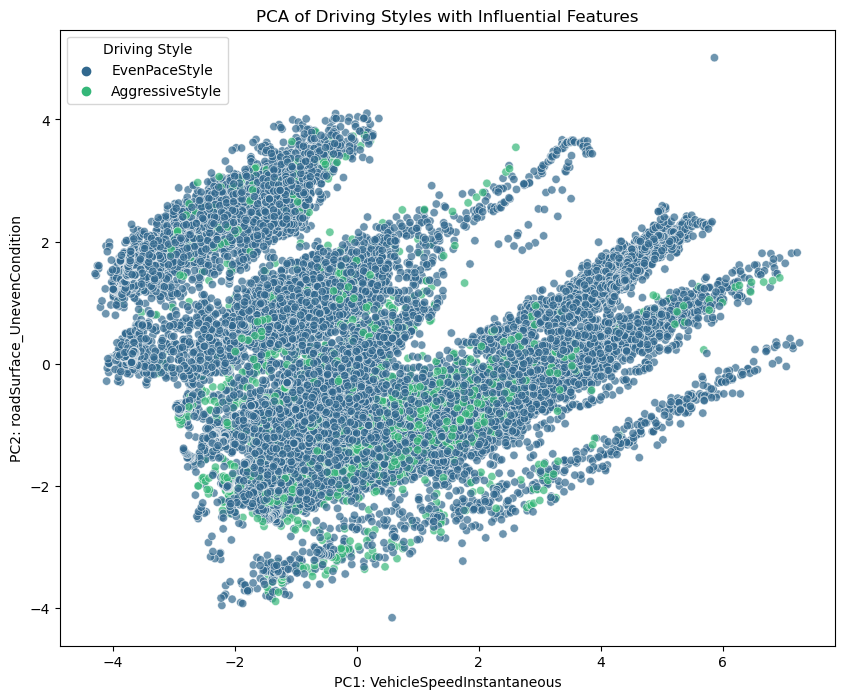
\includegraphics[width=0.8\textwidth]{images/pca_chart.png}
    \caption{PCA Visualization of the Data}
    \label{fig:pca}
\end{figure}

Figure \ref{fig:pca} shows the PCA visualization of the data. The data is not linearly separable, and the classes are not well separated. This suggests that the data is not
linearly separable and that a linear model may not be the best choice for this dataset.
The axes are labelled as PC1: VehicleSpeedInstantaneous and PC2: RoadSurface\_UnevenCondition, which implies that these two features contributes most to the variance in the data.
VehicleSpeedInstantaneous might be defining characteristic of the driving style, while RoadSurface\_UnevenCondition might also influence the driving style.
Despite some level of separation, there is also a significant overlap between the classes, which indicates that not all driving style characteristics are captured by these two features, or there
may be a wide range of behaviours  within each style that could cause this overlap.
The presence of clusters in the data suggests potential for classification models to predict the driving style based on the features.



